\section{LEVEL 5 · De normale verdeling als model}

\begin{missie}
Missie: tem je data met de beroemde klokvorm. (LPD 13)
\end{missie}

\begin{doel}
\textbf{DOEL} \quad Na dit level kan je:

☐ de \textbf{Gausskromme} beschrijven en de betekenis van $\mu$ en $\sigma$ in de kromme uitleggen;

☐ \textbf{grafisch beoordelen} of de normale verdeling een goed model is voor gegeven data;

☐ $\mu$ en $\sigma$ \textbf{schatten} met het gemiddelde $\overline{x}$ en de standaardafwijking $s$ van de data;

☐ de \textbf{68 – 95 – 99,7-regel} gebruiken.
\end{doel}

\subsection*{Theorie 5.1 · Van histogram naar Gausskromme}

\begin{theorie}
Een variabele die je \textbf{meet} (zoals lengte, gewicht of tijd) is \textbf{continu}: ze kan elke waarde in een interval aannemen. Bij veel gegevens en smalle klassen gaat de bovenkant van een histogram naar een vloeiende, klokvormige lijn: de \textbf{Gausskromme}. Het bijhorende model heet de \textbf{normale verdeling}. Je schrijft: $X\sim N(\mu,\sigma)$.

Kenmerken van de Gausskromme:

\begin{itemize}
\item De kromme is \textbf{klokvormig} en \textbf{symmetrisch} rond de lijn $x=\mu$.
\item De top ligt bij $\mu$: gemiddelde, mediaan en modus zijn (ongeveer) gelijk.
\item De kromme raakt de $x$-as nooit, maar komt er ver van $\mu$ heel dicht bij.
\item De \textbf{totale oppervlakte} onder de kromme is 1 (= 100 \%).
\item $\mu$ bepaalt de \textbf{plaats} van de kromme. $\sigma$ bepaalt de \textbf{breedte}: de afstand van $\mu$ tot de \textbf{buigpunten} (de punten waar de kromme van hol naar bol wisselt) is gelijk aan $\sigma$.
\end{itemize}
\end{theorie}

\begin{center}
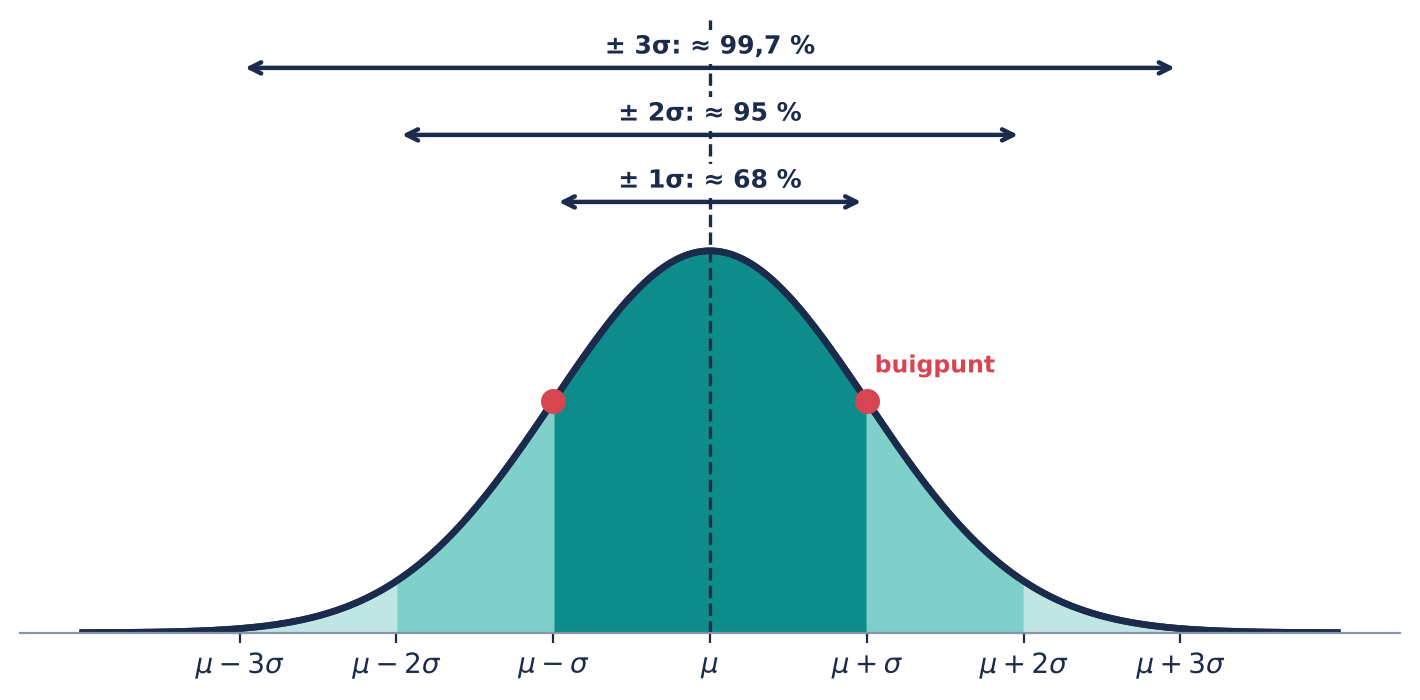
\includegraphics[width=0.85\textwidth]{figuren/l5_gauss_regel.png}
\end{center}

\begin{theorie}
\textbf{De 68 – 95 – 99,7-regel.} Bij een normaal verdeelde variabele liggen ongeveer:

\begin{itemize}
\item \textbf{68 \%} van de waarden in $[\mu-\sigma,\;\mu+\sigma]$;
\item \textbf{95 \%} van de waarden in $[\mu-2\sigma,\;\mu+2\sigma]$;
\item \textbf{99,7 \%} van de waarden in $[\mu-3\sigma,\;\mu+3\sigma]$.
\end{itemize}

Door de symmetrie ligt telkens de helft van het resterende percentage links en de andere helft rechts.
\end{theorie}

\begin{voorbeeld}
\textbf{Voorbeeld.} De lengte van 12-jarige meisjes is bij benadering normaal verdeeld met $\mu=152$ cm en $\sigma=7$ cm.

\begin{itemize}
\item Ongeveer 68 \% van de meisjes is tussen $152-7=145$ cm en $152+7=159$ cm groot.
\item Ongeveer 95 \% is tussen $152-14=138$ cm en $152+14=166$ cm groot.
\item Buiten die 95 \% valt 5 \%; dus ongeveer 2,5 \% is kleiner dan 138 cm en 2,5 \% is groter dan 166 cm.
\end{itemize}
\end{voorbeeld}

\subsection*{Theorie 5.2 · Invloed van $\mu$ en $\sigma$}

\begin{theorie}
\begin{itemize}
\item Verandert $\mu$ (met dezelfde $\sigma$)? De kromme \textbf{verschuift} naar links of rechts, de vorm blijft hetzelfde.
\item Wordt $\sigma$ groter (met dezelfde $\mu$)? De kromme wordt \textbf{breder en lager}. Wordt $\sigma$ kleiner, dan wordt de kromme \textbf{smaller en hoger}.
\item De oppervlakte onder de kromme blijft altijd 1.
\end{itemize}
\end{theorie}

\subsection*{Theorie 5.3 · Is de normale verdeling een goed model?}

\begin{theorie}
Bij gegeven data ga je zo te werk:

\begin{enumerate}
\item \textbf{Beoordeel grafisch} (histogram): is het histogram ongeveer \emph{klokvormig} en \emph{symmetrisch}, met één top en zonder uitschieters? Is $\overline{x}\approx \text{Med}\approx \text{Mod}$?
\item \textbf{Schat de parameters}: $\mu\approx\overline{x}$ en $\sigma\approx s$ (rekenkundig gemiddelde en standaardafwijking van de data).
\item Gebruik het model $N(\overline{x},s)$ om uitspraken te doen over de populatie.
\end{enumerate}

Een normale verdeling past \textbf{niet} bij data die \emph{scheef} zijn (bv. inkomens), \emph{twee toppen} hebben of \emph{vlak} zijn (bv. een dobbelsteen).
\end{theorie}

\subsection*{Aan de slag}

\subsubsection*{Oefening 5.1 \quad ★☆☆ \quad Invullen: de Gausskromme}

\textbf{Woordenlijst:} klokvormig – symmetrisch – $\mu$ – $\sigma$ – buigpunten – 1 – breder – verschuift.

De Gausskromme is \gat{klokvormig} en \gat{symmetrisch} rond de verticale lijn door het gemiddelde. De positie van de top wordt bepaald door \gat{$\mu$}. De afstand van de top tot de \gat{buigpunten} is gelijk aan \gat{$\sigma$}. De totale oppervlakte onder de kromme is \gat{1}. Als $\sigma$ groter wordt, wordt de kromme \gat{breder}; als $\mu$ verandert, \gat{verschuift} de kromme.

\subsubsection*{Oefening 5.2 \quad ★☆☆ \quad De kromme aflezen}

Het gewicht van jongeren in een sportkamp is normaal verdeeld.

\begin{center}
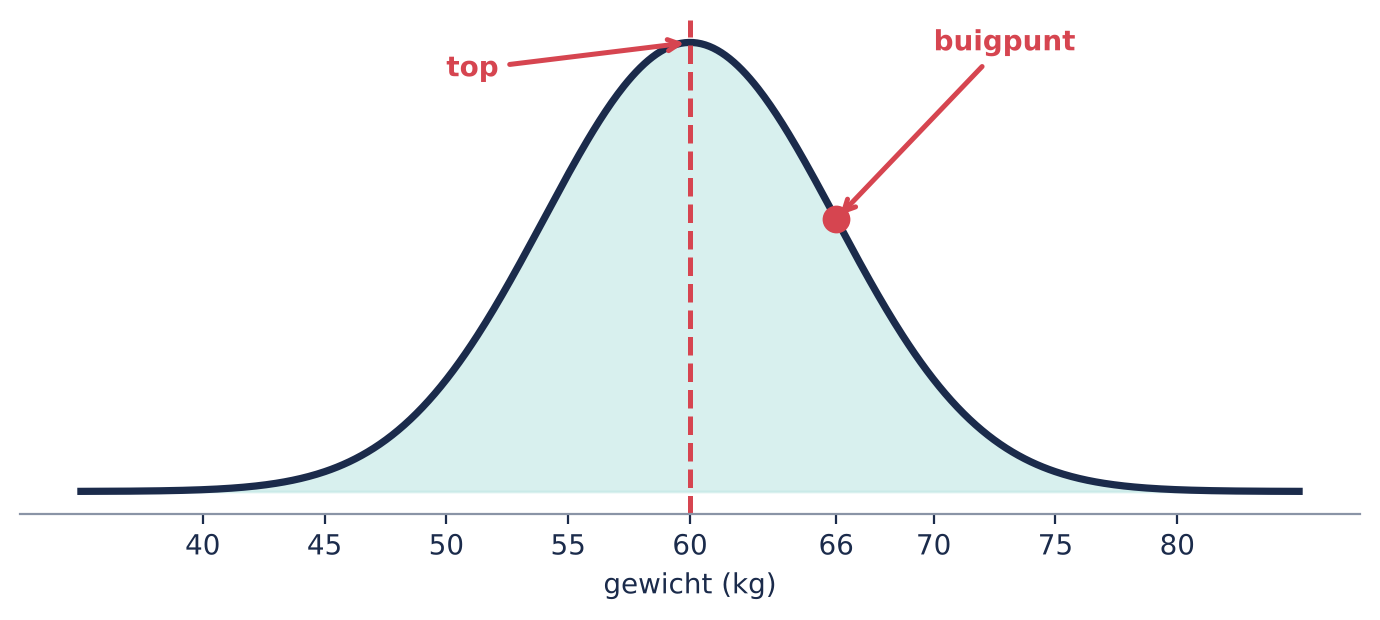
\includegraphics[width=0.8\textwidth]{figuren/l5_aflezen.png}
\end{center}

\textbf{a)} Lees $\mu$ af. \quad \textbf{b)} Lees $\sigma$ af (denk aan het buigpunt). \lijn

\textbf{c)} Tussen welke twee gewichten liggen ongeveer 68 \% van de jongeren? En 95 \%? \lijn

\textbf{d)} Hoeveel procent weegt meer dan 66 kg? \lijn

\begin{oplossing}
\textbf{Oplossing 5.2}

a) $\mu=60$ kg (de top). b) Het buigpunt ligt bij 66, dus $\sigma=66-60=6$ kg. c) 68 \%: tussen 54 en 66 kg; 95 \%: tussen 48 en 72 kg. d) Buiten de 68 \% valt 32 \%, dus 16 \% links en 16 \% rechts: ongeveer 16 \% weegt meer dan 66 kg.
\end{oplossing}

\subsubsection*{Oefening 5.3 \quad ★★☆ \quad Koppel: drie krommen vergelijken}

De grafiek toont drie normale verdelingen A, B en C.

\begin{center}
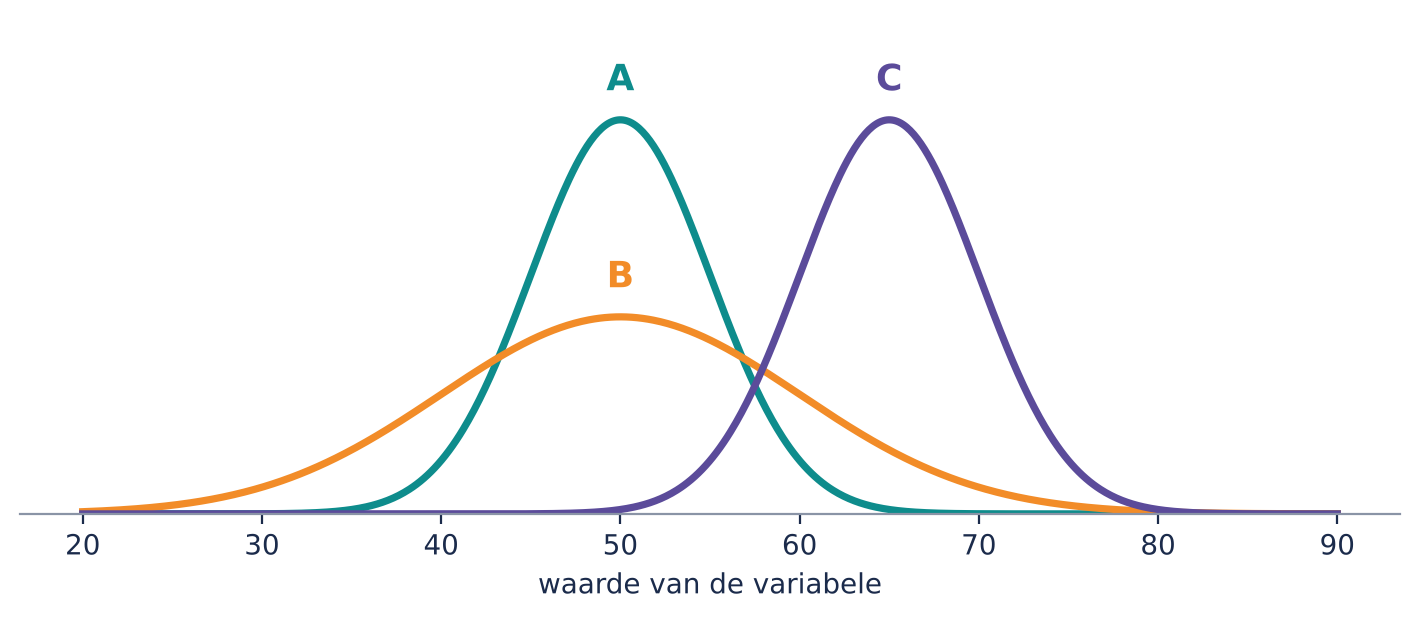
\includegraphics[width=0.8\textwidth]{figuren/l5_mu_sigma.png}
\end{center}

\textbf{a)} Noteer bij benadering $\mu$ voor A, B en C. \lijn

\textbf{b)} Welke twee krommen hebben hetzelfde gemiddelde? Welke hebben dezelfde standaardafwijking? \lijn

\textbf{c)} Welke kromme heeft de grootste standaardafwijking? Hoe zie je dat? \lijn

\textbf{d)} Wat is de oppervlakte onder elke kromme? \lijn

\begin{oplossing}
\textbf{Oplossing 5.3}

a) A: 50; B: 50; C: 65. b) A en B hebben hetzelfde gemiddelde (50). A en C hebben dezelfde standaardafwijking (even breed, namelijk 5). c) B: ze is het breedst en het laagst (σ = 10). d) Voor elke kromme is de oppervlakte 1.
\end{oplossing}

\subsubsection*{Oefening 5.4 \quad ★★☆ \quad Context: past het model?}

Beoordeel voor elk histogram of een normale verdeling een goed model is. Gebruik de grafiek én de kengetallen.

\begin{center}
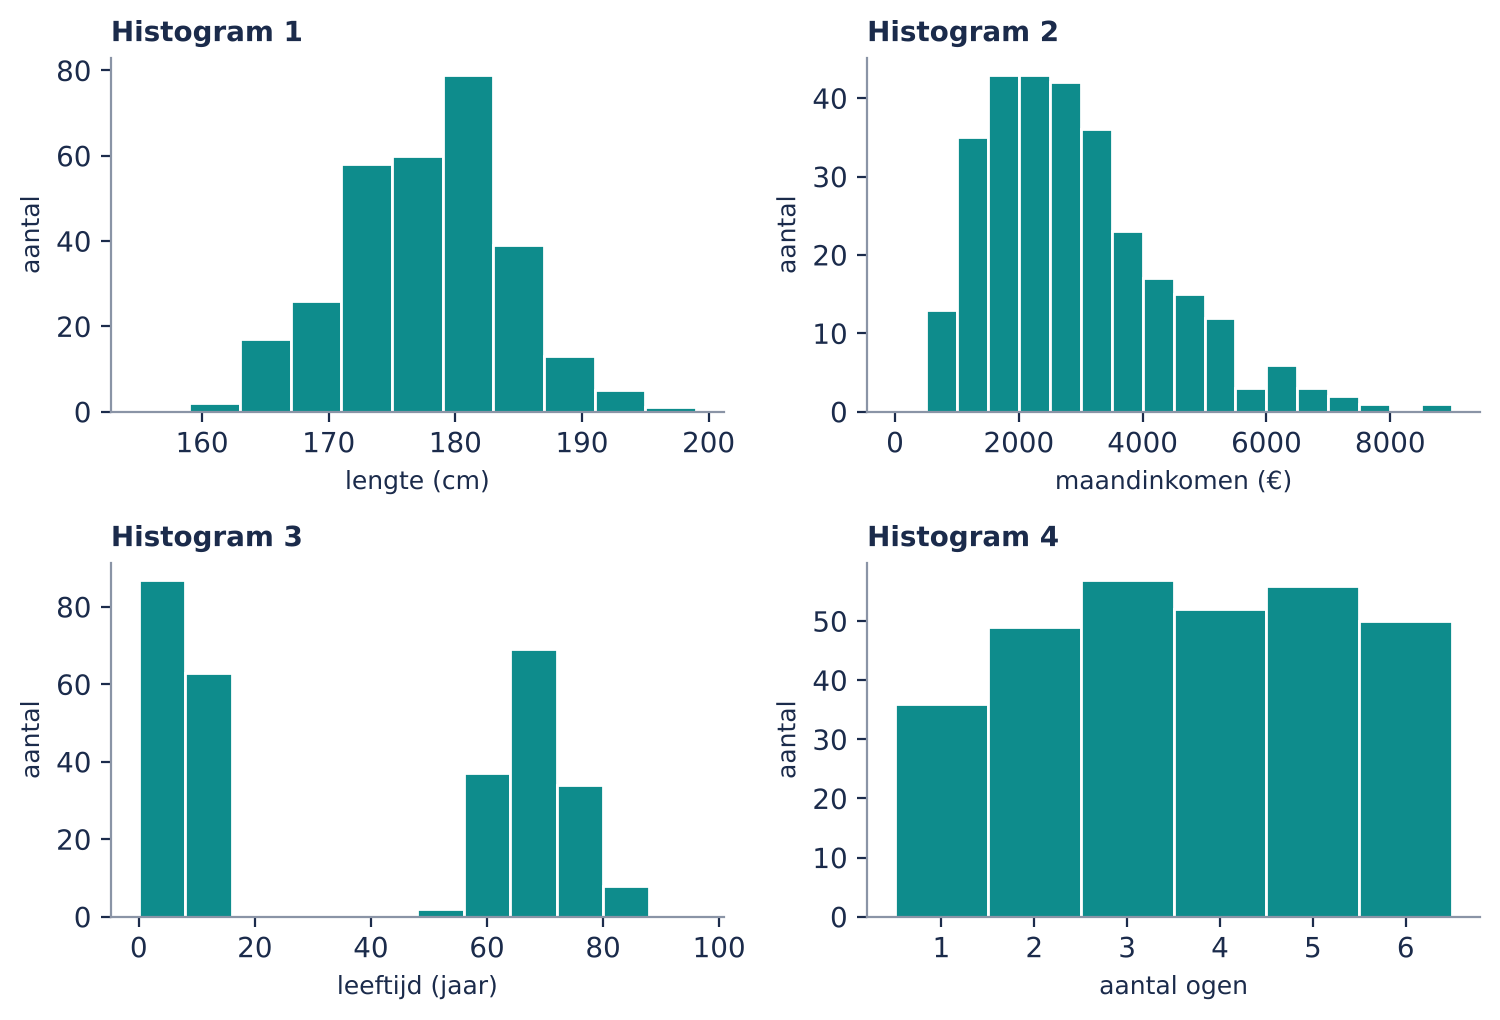
\includegraphics[width=0.95\textwidth]{figuren/l5_histogrammen.png}
\end{center}

\breedtes{30/20/15/15/20}
\begin{tabular}{lcccc}
\hline
Histogram & gemiddelde & mediaan & standaardafwijking & normaal model? \\
\hline
1. lengte van 300 jongens van 17 jaar & 177,2 cm & 177 cm & 6,4 cm & \\
2. maandinkomen van 300 gezinnen & 3\,060 € & 2\,750 € & 1\,946 € & \\
3. leeftijd van 300 bezoekers van een kinderboerderij (kinderen én grootouders) & 37,7 jaar & 31,5 jaar & 30,9 jaar & \\
4. aantal ogen bij 300 worpen met een dobbelsteen & 3,6 & 4 & 1,6 & \\
\hline
\end{tabular}

\begin{oplossing}
\textbf{Oplossing 5.4}

1. Ja: klokvormig, symmetrisch, gemiddelde $\approx$ mediaan. 2. Nee: rechts scheef (lange staart naar hoge inkomens), gemiddelde veel groter dan de mediaan. 3. Nee: twee toppen (kinderen en grootouders); het gemiddelde ligt in een gebied waar bijna niemand zit. 4. Nee: vlak (uniform), alle uitkomsten even waarschijnlijk, geen klokvorm; bovendien discreet.
\end{oplossing}

\subsubsection*{Oefening 5.5 \quad ★★★ \quad ICT: een model opstellen}

Een kinderconsultatiebureau meet de lengte (in cm) van 30 kinderen van 12 maanden:

74,6 – 76,5 – 71,8 – 74,2 – 73,1 – 74,8 – 75,0 – 77,5 – 72,8 – 74,3 – 75,7 – 76,6 – 71,7 – 74,0 – 72,7 – 79,5 – 69,3 – 78,0 – 74,2 – 77,0 – 68,2 – 75,7 – 70,3 – 71,7 – 73,6 – 73,2 – 75,9 – 71,0 – 73,3 – 72,0

\begin{center}
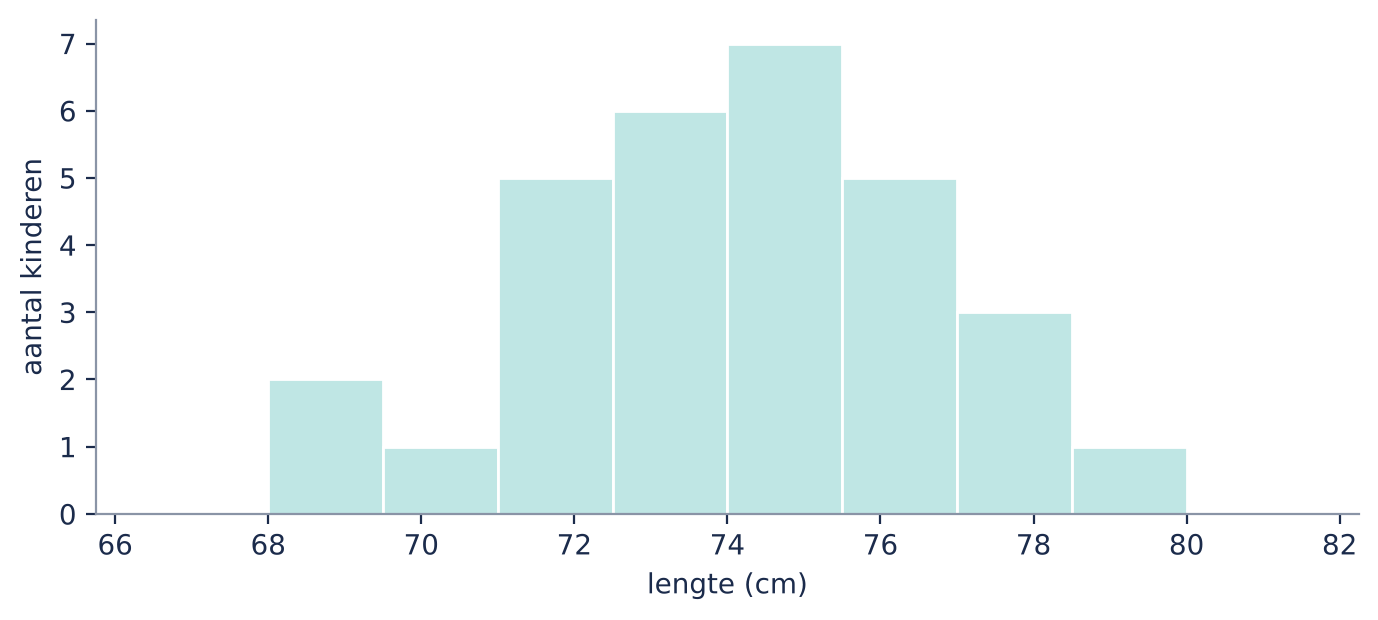
\includegraphics[width=0.75\textwidth]{figuren/l5_baby_histogram.png}
\end{center}

\textbf{a)} Is de normale verdeling een goed model? Verklaar met het histogram. \lijn

\textbf{b)} Bereken met ICT $\overline{x}$ en $s$ en noteer het model $N(\mu,\sigma)$. \lijn

\textbf{c)} Bereken de grenzen $\overline{x}-s$ en $\overline{x}+s$ en tel hoeveel van de 30 lengtes daartussen liggen. Komt het percentage overeen met de 68 \%-regel? \lijn

\textbf{d)} Tussen welke lengtes liggen volgens het model ongeveer 95 \% van de kinderen van 12 maanden? \lijn

\begin{oplossing}
\textbf{Oplossing 5.5}

a) Ja: het histogram is klokvormig en bijna symmetrisch, met één top; de mediaan (74,1) ligt dicht bij het gemiddelde (73,94). b) $\overline{x}\approx 73{,}94$ cm en $s\approx 2{,}59$ cm, dus het model is $N(73{,}94;\,2{,}59)$. c) Grenzen: $71{,}35$ en $76{,}53$; hiertussen liggen 21 van de 30 lengtes ($70\,\%$), dat is dicht bij 68 \%. d) $\overline{x}\pm 2s$: tussen ongeveer 68,8 cm en 79,1 cm (in de data liggen 28 van de 30 in dat bereik, ongeveer 93 \%).
\end{oplossing}

\subsubsection*{Oefening 5.6 \quad ★★☆ \quad De 68 – 95 – 99,7-regel toepassen}

\textbf{a)} De IQ-score is normaal verdeeld met $\mu=100$ en $\sigma=15$. Bereken de percentages van de mensen met een score in: $[85,115]$, $[70,130]$ en $[55,145]$. \lijn

\textbf{b)} Hoeveel procent heeft een IQ boven 115? En boven 130? \lijn

\textbf{c)} De slaapduur van tieners is bij benadering normaal verdeeld met $\mu=8{,}0$ uur en $\sigma=1{,}0$ uur. Hoeveel procent slaapt minder dan 6 uur? Schrijf een antwoordzin. \lijn

\begin{oplossing}
\textbf{Oplossing 5.6}

a) $[85,115]=[\mu-\sigma,\mu+\sigma]$: 68 \%; $[70,130]=[\mu-2\sigma,\mu+2\sigma]$: 95 \%; $[55,145]=[\mu-3\sigma,\mu+3\sigma]$: 99,7 \%. b) Boven 115: $\dfrac{100-68}{2}=16$ \%. Boven 130: $\dfrac{100-95}{2}=2{,}5$ \%. c) 6 uur $=\mu-2\sigma$; onder $\mu-2\sigma$ ligt 2,5 \%. Antwoordzin: ongeveer 2,5 \% van de tieners slaapt minder dan 6 uur.
\end{oplossing}

\subsubsection*{Oefening 5.7 \quad ★★★ \quad Foutjager}

\textbf{1.} Zara: ‘Bij een normale verdeling is $\sigma$ de afstand van $\mu$ tot het einde van de kromme.’ \lijn

\textbf{2.} Milan: ‘Als $\sigma$ groter wordt, wordt de oppervlakte onder de kromme ook groter.’ \lijn

\textbf{3.} Fien: ‘Mijn histogram heeft twee toppen, maar $\overline{x}$ en $s$ kan ik toch berekenen, dus de normale verdeling past.’ \lijn

\begin{oplossing}
\textbf{Oplossing 5.7}

1. Fout: $\sigma$ is de afstand van $\mu$ tot een buigpunt; de kromme loopt oneindig door. 2. Fout: de oppervlakte is altijd 1; de kromme wordt breder en lager. 3. Fout: $\overline{x}$ en $s$ kan je altijd berekenen, maar een model met twee toppen is niet klokvormig; de normale verdeling past dan niet.
\end{oplossing}

\subsection*{CHECK · Level 5}

\textbf{1.} (2 p) Noem drie kenmerken van de Gausskromme. \lijn

\textbf{2.} (2 p) Een normale verdeling heeft top bij 40 en een buigpunt bij 45. Noteer $\mu$ en $\sigma$. \lijn

\textbf{3.} (2 p) Een histogram is rechts scheef met $\overline{x}=48$ en $\text{Med}=39$. Is een normaal model geschikt? Verklaar. \lijn

\textbf{4.} (2 p) De duur van een bezoek is normaal verdeeld met $\mu=35$ min en $\sigma=6$ min. Tussen welke waarden liggen ongeveer 68 \% van de bezoeken? \lijn

\begin{doel}
\textbf{Score:} \_\_\_ / 8 \quad ☐ behaald (vanaf 5 / 8) \quad ☐ nog even oefenen
\end{doel}

\begin{oplossing}
\textbf{Oplossing CHECK 5}

1. Klokvormig, symmetrisch, top bij $\mu$, totale oppervlakte 1 (ook: buigpunten op afstand $\sigma$). 2. $\mu=40$ en $\sigma=45-40=5$. 3. Nee: de verdeling is scheef en gemiddelde en mediaan liggen ver uit elkaar. 4. Tussen $35-6=29$ en $35+6=41$ minuten.
\end{oplossing}
